\documentclass[reprint,amsmath,amssymb,aps,prb]{revtex4-2}

\usepackage{graphicx}% Include figure files
\usepackage{dcolumn}% Align table columns on decimal point
\usepackage{bm}% bold math
\usepackage{hyperref}% add hypertext capabilities
\usepackage{xcolor}
\usepackage{braket}
\usepackage[english]{babel}

%% Philipps stuff %%
\usepackage[font={small}]{caption}
\usepackage{subcaption}
\captionsetup[subfigure]{list=true, font=small, labelfont=bf, 
	labelformat=brace, position=top}
\usepackage{amsmath}
\def\arraystretch{1.5}
\usepackage{float}
\usepackage{lipsum}


%% Code stuff %%
\usepackage{listings} % insert code fragments

\definecolor{codegreen}{rgb}{0,0.6,0}
\definecolor{codegray}{rgb}{0.5,0.5,0.5}
\definecolor{codepurple}{rgb}{0.58,0,0.82}
\definecolor{backcolour}{rgb}{0.95,0.95,0.92}

\lstdefinestyle{mystyle}{
    backgroundcolor=\color{backcolour},   
    commentstyle=\color{codegreen},
    keywordstyle=\color{magenta},
    numberstyle=\tiny\color{codegray},
    stringstyle=\color{codepurple},
    basicstyle=\ttfamily\footnotesize,
    breakatwhitespace=false,         
    breaklines=true,                 
    captionpos=b,                    
    keepspaces=true,                 
    numbers=left,                    
    numbersep=5pt,                  
    showspaces=false,                
    showstringspaces=false,
    showtabs=false,                  
    tabsize=2
}

\lstset{style=mystyle}

\begin{document}

%\title{Project title}

\author{Your Name}

\date{\today}% It is always \today, today,
             %  but any date may be explicitly specified

\begin{abstract}
A paper usually includes an abstract, a concise summary of the work covered at length in the main body of the paper. Please also write a short abstract of your project.
\end{abstract}


\maketitle




\section{Guidelines}



Please write a short paper about your project. There are no strict length limits, but please write \textbf{at least two pages in the layout of this template} (including figures, excluding references and code listings). Please structure your paper in a scientific way, and include your references and your code. There are \LaTeX packages you can use to preserve the indentation of your code, e.g. the \texttt{listings} package which is demonstrated in the Appendix~\ref{app:codes}.

This sample document makes use of of REV\TeX~4.2, therefore you will need to install it to be able to compile this document yourself. Further information can be found in the REV\TeX~4.2
documentation included in the distribution or available at
\url{http://journals.aps.org/revtex/}.



\subsection{Example citations}
By default, citations are numerical\cite{epr}, some more citations~\cite{feyn54,Bire82,Berman1983,witten2001,Davies1998}. 

\subsection{Exampe figure}
Including and referring to figures is as usual, see for instance Fig.~\ref{fig:example}
\begin{figure}
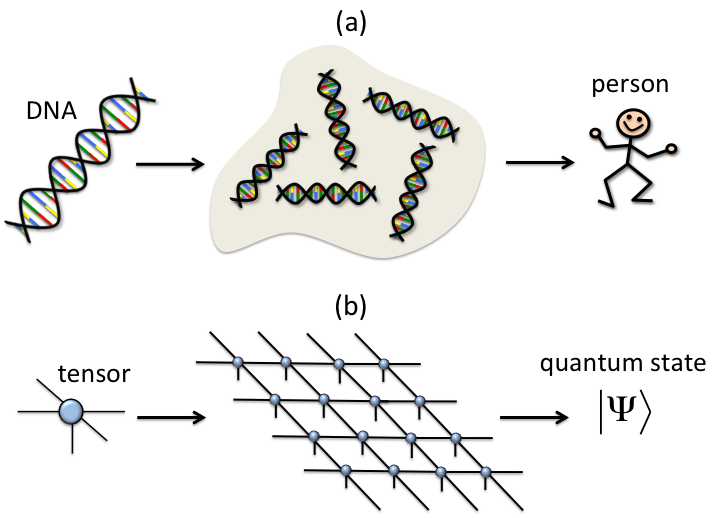
\includegraphics[width=0.99\linewidth]{cartoon.png}
\caption{Example of a figure~\cite{Orus2013}.}
\label{fig:example}
\end{figure}

\bibliography{bibsamp}% Produces the bibliography via BibTeX.


\appendix


\begin{widetext}
\section{Code listing} \label{app:codes}
Please copy your code in the appendix.
\begin{lstlisting}[language=Python]
"""

Module to generate the Hamiltonian of the transverse field Ising model.

H = -J sum_i sigma^x_i sigma^x_{i+1} - g sum_i sigma^z i.

Used in the solution of exercise 5.1

"""

import numpy as np
import scipy
from scipy import sparse
import scipy.sparse.linalg
import matplotlib.pyplot as plt

Id = sparse.csr_matrix(np.eye(2))
Sx = sparse.csr_matrix([[0., 1.], [1., 0.]])
Sz = sparse.csr_matrix([[1., 0.], [0., -1.]])
Splus = sparse.csr_matrix([[0., 1.], [0., 0.]])
Sminus = sparse.csr_matrix([[0., 0.], [1., 0.]])


def singesite_to_full(op, i, L):
    op_list = [Id]*L  # = [Id, Id, Id ...] with L entries
    op_list[i] = op
    full = op_list[0]
    for op_i in op_list[1:]:
        full = sparse.kron(full, op_i, format="csr")
    return full


def gen_sx_list(L):
    return [singesite_to_full(Sx, i, L) for i in range(L)]


def gen_sz_list(L):
    return [singesite_to_full(Sz, i, L) for i in range(L)]


def gen_hamiltonian_periodic(sx_list, sz_list, g, J=1.):
    """ assumes periodic boundery conditions """
    L = len(sx_list)
    H = sparse.csr_matrix((2**L, 2**L))
    for j in range(L):
        H = H - J *( sx_list[j] * sx_list[(j+1)%L])
        H = H - g * sz_list[j]
    return H
\end{lstlisting}
\end{widetext}

\title{Machine Learning of Many Body Localization}

\author{Philipp Krüger}

\date{\today}% It is always \today, today,
             %  but any date may be explicitly specified

\begin{abstract}
The goal of this study was to find the quantum phase transition at intermediate local disorder strengths on a Heisenberg chain. Exact diagonalization was used to find the reduced density matrices for a different number of consecutive spins for the lowest energy eigenstate of the Heisenberg model with an additional random field in z-direction at low and high disorder strengths. The resulting dataset representing extended and localized phases was used to train a neural network. Afterwards, the trained network was applied on intermediate disorder strengths to deduct the critical disorder strength for a phase transition. This phase transition was predicted for all system sizes to be around $W_c = 2.5 J$ for the system sizes $L\in\{8, 9, 10, 11, 12\}$ and block sizes $n\in\left[1,6\right]$. Low block and system sizes suffered from low accuracy and high losses in the machine learning model, whereas for $n>3$ block sizes the $W_c$ value showed smaller deviations from a previously published theoretical value $W_c\approx3.6$ calculated with entanglement entropy on systems up to $L=22$. This deviation can be attributed to the effect of the smaller system sizes and the effect of open boundary conditions.
\end{abstract}

\maketitle

\section{Introduction}

The physical model and the concept of exact diagonalization is presented first. As we use reduced density matrices as features for the neural network, we explain briefly their computation and meaning.
%Review Literature on task. How other people find $W_c$?
%Why is the topic interesting? => Finding Wc?
\subsection{Physical model}

\subsubsection{Hamiltonian of the Heisenberg model and physical expectation}

The Hamiltonian of the Heisenberg model is shown in equation \ref{hamiltonian}. In the course of further analysis, we choose $J=1$ and sample $h$ from a uniform distribution such that $h_i \in \left[-W, W\right]$.

\begin{equation}
	H=\underbrace{J\sum_i \vec{S}_i\cdot\vec{S}_{i+1}}_{\text{Exchange Energy}}-\underbrace{\sum_ih_iS_i^z}_{\text{Random Field}}\label{hamiltonian}
\end{equation}

The expectation for the ground state is dependent on the ratio of the coupling and the local random field. 

For $\frac{W}{J} \ll 1$, we expect a delocalized, extended phase, since the exchange energy dominates over the small external field. Therefore, the system can relax to thermal equilibrium serving as its own heat bath in the limit of large system size $L\rightarrow\infty$.
Here, the reduced density operator of a finite subsystem converges to the equilibrium thermal distribution
for $L\rightarrow\infty$.\cite{Pal2010}

For $\frac{W}{J} \gg 1$, we can expect a localized phase, since the $h_i$ factors dominate over the exchange energy. The resulting states are expected to be product states of spins "up" or "down", as the external field points in z-direction. Also, an infinite system cannot equilibrate itself. The local configurations are set by the initial conditions at all times and are adiabatically connected to the trivial state.\cite{Pal2010}

\subsubsection{Characterization of ergodic and localized regimes by different metrics}

There are a few different ways of how to distinguish the ergodic and the localized regime by accessible metrics. 
One can study spectral analysis, where the ergodic states are distributed like a Gaussian Orthogonal Ensemble (GOE), and the localized states follow a Poisson distribution.\cite{Laumann2014}

Another interesting metric is the entaglement entropy, which indicates the information spread between different system parts.\cite{Nandkishore_2015} In the ergodic phase, the reduced density matrix $\rho_A$ of a ground state is expected to be thermal. This leads to a volume law scaling for the entanglement entropy.\cite{Altman_2015}	On the other hand, localized eigenstates show area-law scaling.\cite{yu2019bulk}
%W—>0 : reduced matrix : thermal density matrix , volume law entanglement
%W —> \infty : reduced density matrix: … , area law entanglement
%n is finite and large enough
%reduced density matrix would be different on two sides.

In this study, we solve the Hamiltonian via exact diagonalization to predict the phase change by training a neural network with low and high disorder strengths, assuming that the resulting reduced density matrices represent an ergodic and localized phase respectively. To access the ground states, previous approaches made use of the shift-invert method \cite{Luitz2015}. The same paper suggests a critical disorder strength of $h_c=3.62$ for the same system by using the evolution of the entanglement entropy over different system sizes as an argument.


%\begin{figure}
%	\centering
%	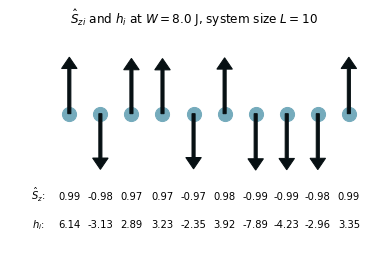
\includegraphics[width=1\linewidth]{figures/heisenberg_chain}
%	\caption{Visualization of the random disorder strength efftect on a ground state.}
%	\label{fig:heisenberg_chain}
%\end{figure}

\subsection{Exact diagonalization}

Exact diagonalization (ED) is a numerical technique we can use to solve the time independent Schrödinger Equation $H\ket{\psi}=E\ket{\psi}$ for the eigenvalues $E$ and eigenvectors $\ket{\psi}$. This only works if the Hamiltonian $H$ represents a discrete and finite system. Most quantum many-particle problems lead to a sparse matrix representation of the Hamiltonian, where only a very small fraction of the matrix
elements is non-zero.\cite{Weisse2008} An efficient method to find ground states is the Lanczos algorithm.\cite{Lanczos1950} At first, the algorithm was numerically unstable. This issue was overcome in 1970 by Ojalvo and Newman.\cite{Ojalvo1970} In this study, we rely on the Lanczos algorithm for the eigensolver.

\subsection{Reduced Density Matrix}

The usefulness of reduced density matrices has already been shown by White in 1992 with ground states of Heisenberg chains.\cite{White1992} In our case we use areal density matrices as features for the neural network to predict the critical disorder strength of a phase change from delocalized to localized. The reduced density matrix is defined in equation \ref{red_density}. Physically, the reduced density matrix $\rho_A$, provides correct measurement statistics for subsystem A.

\begin{eqnarray}
\rho_{AB}&=&\ket{\psi_A}\bra{\psi_A}\otimes\ket{\psi_B}\bra{\psi_B}\\
\rho_A&=&\text{Tr}_B(\rho_{AB})=\ket{\psi_A}\bra{\psi_A}\text{Tr}\left(\ket{\psi_B}\bra{\psi_B}\right)\label{red_density}
\end{eqnarray}%\url{http://www.thphys.nuim.ie/staff/jvala/Lecture_9.pdf}

The reduced density matrix was also used by Zhang in 2019 to learn the localization transition in disordered quantum Ising spin chains. Here, the motivation was to reduce the dimension and filter out redundant information. However, it proved to be inferior in comparison to the full density matrix in the analysis.\cite{Zhang2019} However, due to RAM limitations, we will rely on reduced density matrices.


\subsection{Artificial Neural Networks}

In 1958, Rosenblatt published his concept of the probabilistic model for information storage and organization in the brain, which greatly inspired others to use those models for computation.\cite{Rosenblatt1958} Over the course of the last decades, they have evolved into a tool that can be used for a variety of applications including computer vision, speech recognition, medical diagnosis, playing games or even artistic painting.\cite{Gatys2015}

The reduced density matrices are essentially complex 2D arrays with length $2^n\times2^n$. As we want to classify for an arbitrary $W$ whether we have a localized or delocalized phase, it is convenient to use a machine learning classifier. The density matrices can then be thought of as a complex and real image that can be fed into it analogously to classical image classification. A prominent tool to use in spatially or temporarly related data is the Convolutional Neural Network, which will be applied here for two reasons: Firstly, they reduce the total number of weights, which is convenient for a low sample size \cite{Schmidhuber2015}. Secondly, the thermalization of the density matrix may be learnable by a convolution kernel because we are expecting the density matrices to show different local distributions.


\section{Computational Methods}

The strategy for implementation was as follows:

\begin{enumerate}
	\item Generate Hamiltonian from random disorder strength and system size. Then calculate lowest eigenstate near Energy $E = 0$.
	\item Generate density matrix from the eigenstate and the respective reduced density matrices for defined block sizes $n$.
	\item  Set up machine learning model per $n$, $L$ that takes density matrices of different $W$ as an input and predicts whether the state represents an extended or a localized phase.
	\item Make predictions for different system sizes L and block sizes $n$ and plot the predictions over $W$. Then extract $W_c$	from the data by using a fit function.
\end{enumerate}

Critical decisions and specifications for each steps are listed below. Afterwards, a brief motivation for the parameter range and resolution is given.

\subsection{Eigenvalue solver and shift invert method}

For the eigenvalue solution, we use SciPy's method \texttt{eigsh}. However, the computation of eigenvalues near zero is computationally very costly and sometimes did not even converge during the standard maximum of iterations. 

Most ARPACK functionalities are included in \texttt{eigsh}. To compute the eigenvalues, we are relying on the so called shift-invert method, which is a mode that allows a quick determination of non-external eigenvalues. This mode involves transforming the eigenvalue problem to an equivalent problem with different eigenvalues. 

In particular, the method is based on the observation that one can find for the generalized eigenvalue problem

\begin{equation}
Ax=\lambda M x
\end{equation}
that
\begin{equation}
\left(A-\sigma M\right)^{-1}Mx = vx, \quad v=\frac{1}{\lambda-\sigma}.
\end{equation}

As we want to find the ground state, our choice for $\sigma$ is zero. The transformed eigenvalues will then satisfy $v=1/\lambda$, so our small eigenvalues  become large eigenvalues for which the Lanczos algorithm converges faster.\cite{Virtanen_2020} This method is also used as part of a efficient phase characterization method by Luitz in 2015.\cite{Luitz2015}

\subsection{Computation of the reduced density matrix}

To get the reduced density matrix of system A, one has to "trace out" all states outside of A. The library QuTiP supplies a method \texttt{ptrace}, which does exactly that. It is important to note that the method takes those indices as an argument which should be kept.\cite{Johansson2012}

A demonstration of the functionality can be found in Figure \ref{fig:partialtrace_proof_of_concept}.

\begin{figure}[h!]
\centering
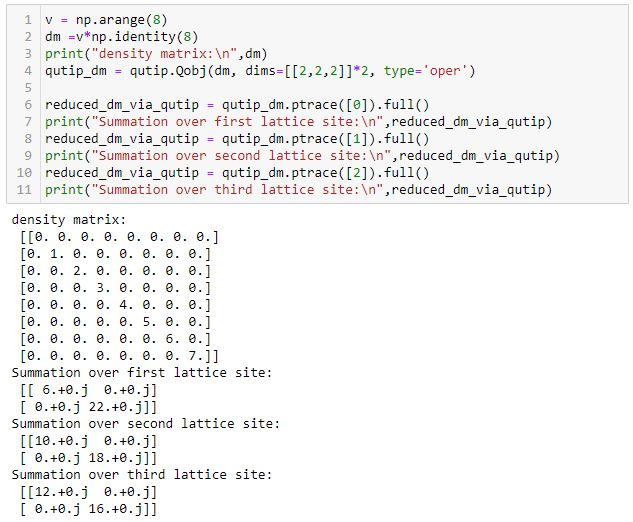
\includegraphics[width=0.7\linewidth]{figures/partialtrace_proof_of_concept}
\caption{Proof of concept for partial trace calculation similar to \protect\hyperlink{http://qutip.org/docs/3.1.0/guide/guide-tensor.html}{QuTiP-Guide/ptrace}.}
\label{fig:partialtrace_proof_of_concept}
\end{figure}

The algorithm of selecting the position vector of $n$ consecutive sites was implemented as follows: 
\begin{enumerate}
	\item Find the center spin rounded to next lowest integer.
	\item Determine left chain length $n_\text{left}$ to be $n/2$, which is rounded to the next lowest integer.
	\item Determine right chain length $n_\text{right}$ as $n-n_\text{left}$.
	\item Select spins from left chain end to right chain end around center spin.
\end{enumerate}
This results in a behavior that picks left indices more favorably, but succeeds if equally spaced ends exist. Let the spins be numbered as $\{1, 2, 3, 4, 5\}$ for $N=5$, then  $n=3$ results in $\{2, 3, 4\}$, whereas $n=2$ results in $\{2, 3\}$.

These lattice sites then serve as an input to the partial trace function, such that the density matrix represents the measurement statistics of the center system.

\subsection{Machine learning models and error metrics}\label{sec:nn}

The decision for the machine learning framework \texttt{keras} was motivated by its flexibility and simplicity.\cite{chollet2015keras}

When setting up the machine learning model, one can already specify the first and last layer: The first (input) layer has to match the sample size of the incoming data, this can be already computed in advance. The length $len$ for block size $n$ is $2\cdot\left(2^n\times 2^n \right)$. The factor 2 comes from a preprocessing step, where the complex values are mapped to a second real picture, since the fitting procedure usually does not expect complex numbers. The last layer is a one node sigmoid, as the target output is the one-dimensional classification in $\left[0,1\right]$.

For small sample sizes, there exist various approaches to choose the right amount of layers and regularization methods, which cannot be generalized, as they heavily depend on feature size and target dimension.\cite{Olson2018,Feng2019}

To balance off the trade between overfitting and loss, the starting point for the model was one hidden layer with 64 nodes. Since the reduced density matrices are similar to image classification and the inspection of the training set indicated that the density matrices had different slopes, a convolutional layer was employed for block sizes of $n<3$, as a $8x8$ picture seemed too small for kernel operations. To compensate the lacking layer, a dense layer of 32 nodes was chosen.

The optimizer Adam was chosen, because it is computationally efficient and
has little memory requirements. \cite{Kingma2014}

For a two label classification problem, it is useful to use cross-entropy as a loss metric, as the penalty increases exponentially the further one deviates from the correct prediction.\cite{Goodfellow-et-al-2016}
\begin{figure}[h!]
\centering
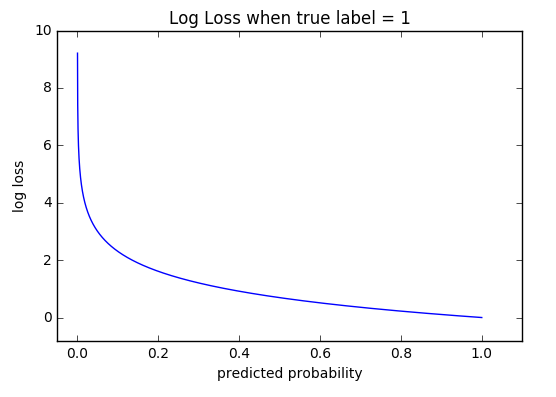
\includegraphics[width=\linewidth]{figures/cross_entropy}
\caption{Example for cross-entropy loss depending on the predicted probability of $\hat{y}=1$.}
\label{fig:cross_entropy}
\end{figure}
The definition for a two class cross-entropy loss can be found in equation \ref{cross-loss}, where $y \in \{0,1\}$ is the true class and $\hat{y}\in\left[0,1\right]$ the predicted probability. This loss is also plotted in Figure \ref{fig:cross_entropy}.
\begin{equation}
L(\hat{y}, y)=-\left(y\log(\hat{y})+(1-y)\log(1-\hat{y})\right)\label{cross-loss}
\end{equation}

\subsection{Extraction of critical disorder strength $W_c$}\label{sec:wcextract}


To fit for the critical disorder strength $W_c$, 180 sample predictions were averaged and plotted over the corresponding disorder strength, for which the test sample was initialized. The first approach was to fit for $W_c$ by using parameters of a fitted linear function or logistic function. As this approach proved to be unstable and not prone to outliers, a far simpler method was employed, which just extracted the nearest guess to $\hat{y}=0.5$, resembling equal prediction probabilities for the localized and ergodic phase.

\begin{lstlisting}[language=Python]
nearest = np.argmin(np.abs(y - 0.5))
\end{lstlisting}


\subsection{Limitations for parameter range and resolution}\label{sec:param}

\begin{enumerate}
	\item System size $L$: Limited by computing time of eigenvalue solver. For the system size $L=12$, one calculation lasted approximately two minutes.
	\item Block size $n$: We go up to $n=6$, which is half of the system size of the biggest system.
	\item Sample size: 2400 samples can be generated for $L=12$, $n_{max}=6$ in approximately 15 hours on the provided machine. Assuming that the whole program should be reproducable in a reasonable time frame, this was found to be a sufficient sample size per system and block size.
	\item Disorder strength $W$ for the testing set: Since each point of a test set comes with a Hamiltonian with randomly drawn $h_i\in\left[-W,W\right]$, a decent amount of variance can be expected for the phase prediction. As we want to extract the phase change in general, and are not interested in the particular phase predictions of one specific Hamiltonian we choose to regularize the prediction by averaging over $180$ predicted samples.
\end{enumerate}

\section{Results}

\subsection{Generation of reduced density matrix training set}

The parameter range for the computation of the reduced density matrices can be found in Table \ref{tab:par_train}. The total computation time was 16.5 h, where 12.5 h where solely needed to compute the ground states of the $L=12$ system.

\begin{table}[h!]
	\centering
	\begin{tabular}{rl}
		\hline
		Parameter & Range or Set \\
		\hline
		\hline 
	\textbf{System size:} & $L \in \{8, 9, 10, 11, 12\}$ \\ 
		\textbf{Block size:} & $n \in \{1, 2, 3, 4, 5, 6\}$ \\ 
		\textbf{Repetitions:} & $r=500$\\
		\hline
	\end{tabular} 
	\caption{Parameter choice for training set generation}\label{tab:par_train}
\end{table}

In order to give some visual intuition, Figures \ref{fig:groundstates_loc} and \ref{fig:groundstates_erg} show realizations for different block sizes and phases.

%\onecolumngrid
\begin{center}
	\begin{figure}[h!]
		\centering	
		\begin{subfigure}[c]{0.45\textwidth}
			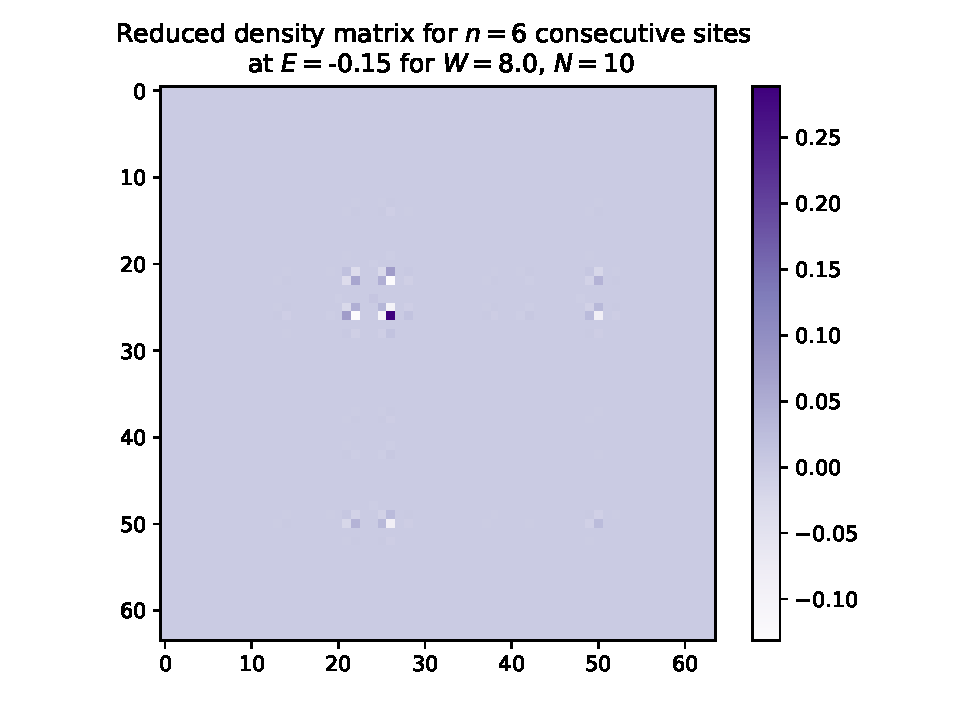
\includegraphics[width=\linewidth]{../results/groundstates/N10n6_trainingset_groundstate_Wmax8.0}
			\subcaption{Visualization of the ground state for a large block size $n=6$ in the localized phase.}
		\end{subfigure}
		\begin{subfigure}[c]{0.45\textwidth}
			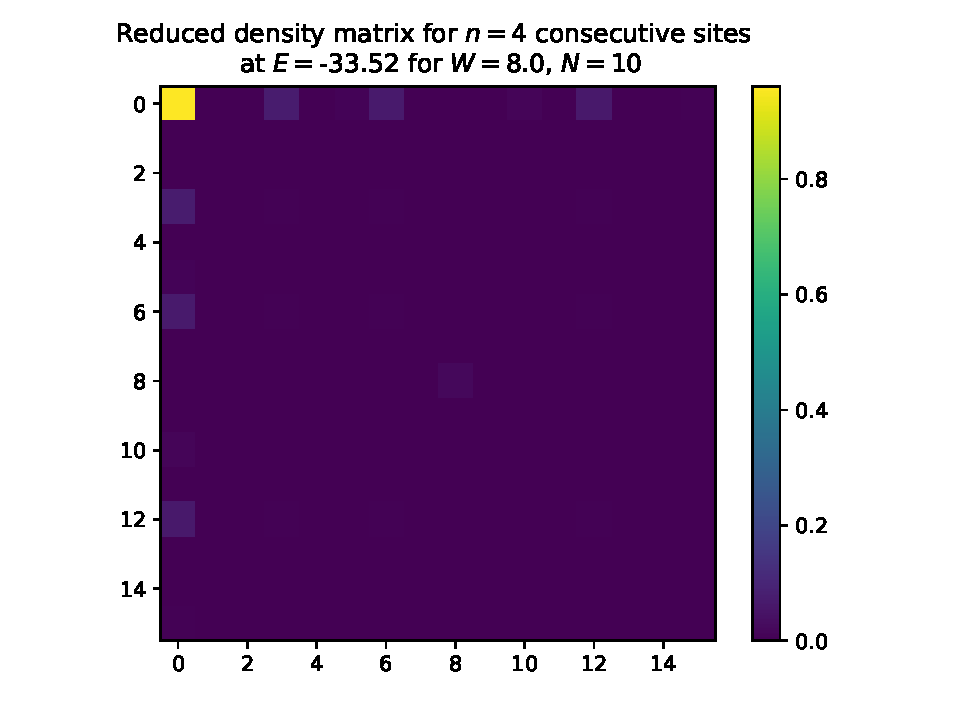
\includegraphics[width=\linewidth]{../results/groundstates/N10n4_trainingset_groundstate_Wmax8.0}
			\subcaption{Visualization of the ground state for an intermediate block size $n=4$ in the localized phase.}
		\end{subfigure}
		\begin{subfigure}[c]{0.45\textwidth}
			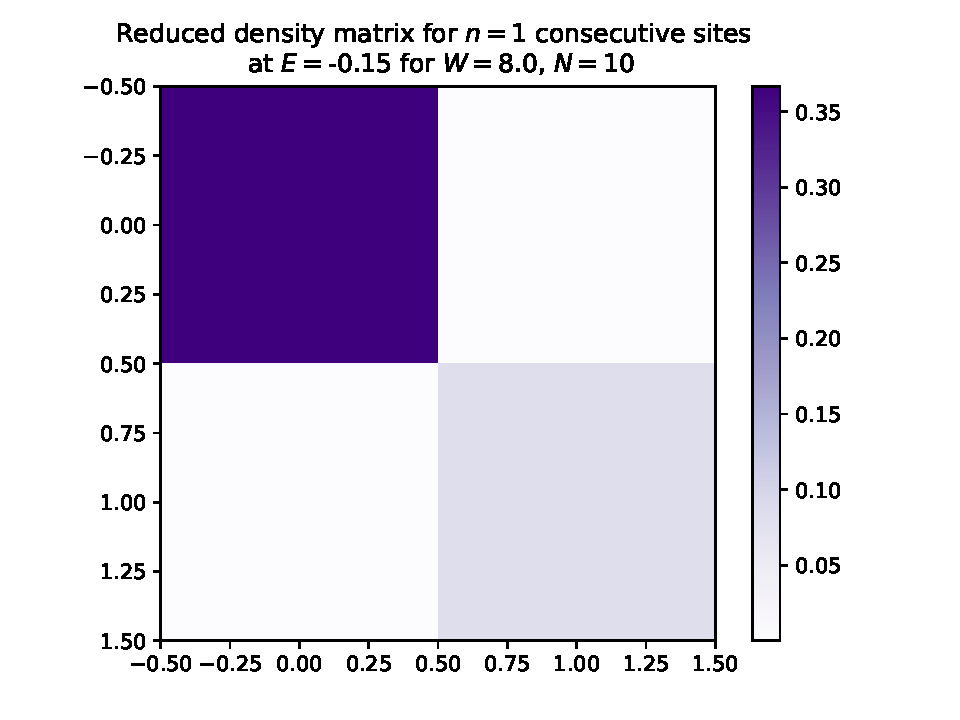
\includegraphics[width=\linewidth]{../results/groundstates/N10n1_trainingset_groundstate_Wmax8.0}
			\subcaption{Visualization of the ground state for the minimal block size $n=1$ in the localized phase.}
		\end{subfigure}
		\caption{Ground states for different block sizes $n$ and phases.}
		\label{fig:groundstates_loc}
\end{figure}
\end{center}
\begin{center}
	\begin{figure}[h!]
		\begin{subfigure}[c]{0.45\textwidth}
			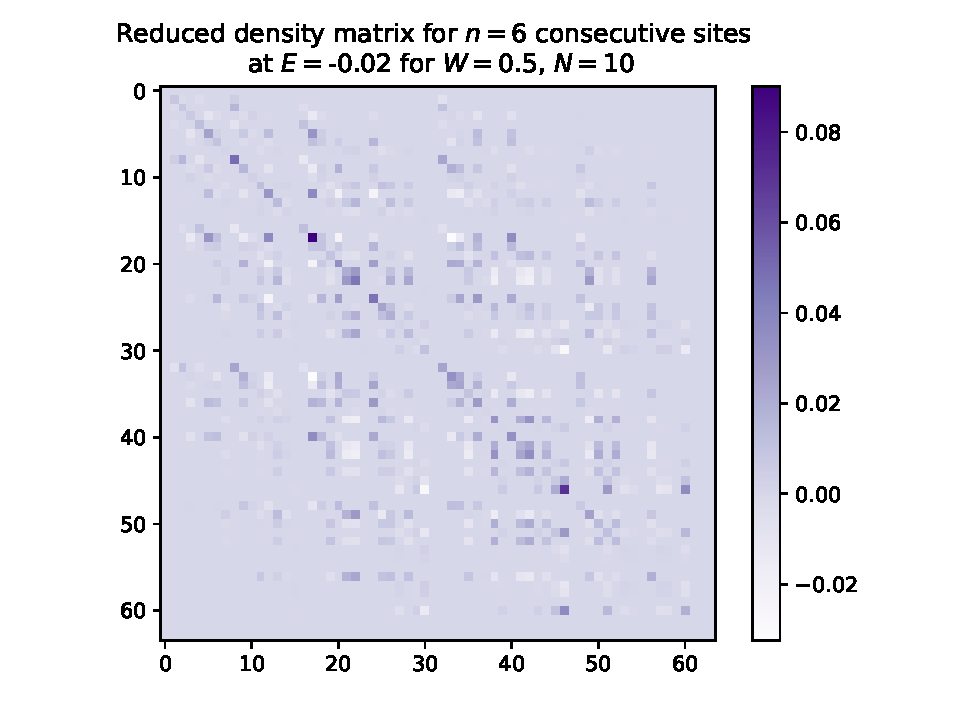
\includegraphics[width=\linewidth]{../results/groundstates/N10n6_trainingset_groundstate_Wmax0.5}
			\subcaption{Visualization of the ground state for a large block size $n=6$ in the ergodic phase.}
		\end{subfigure}
		\begin{subfigure}[c]{0.45\textwidth}
			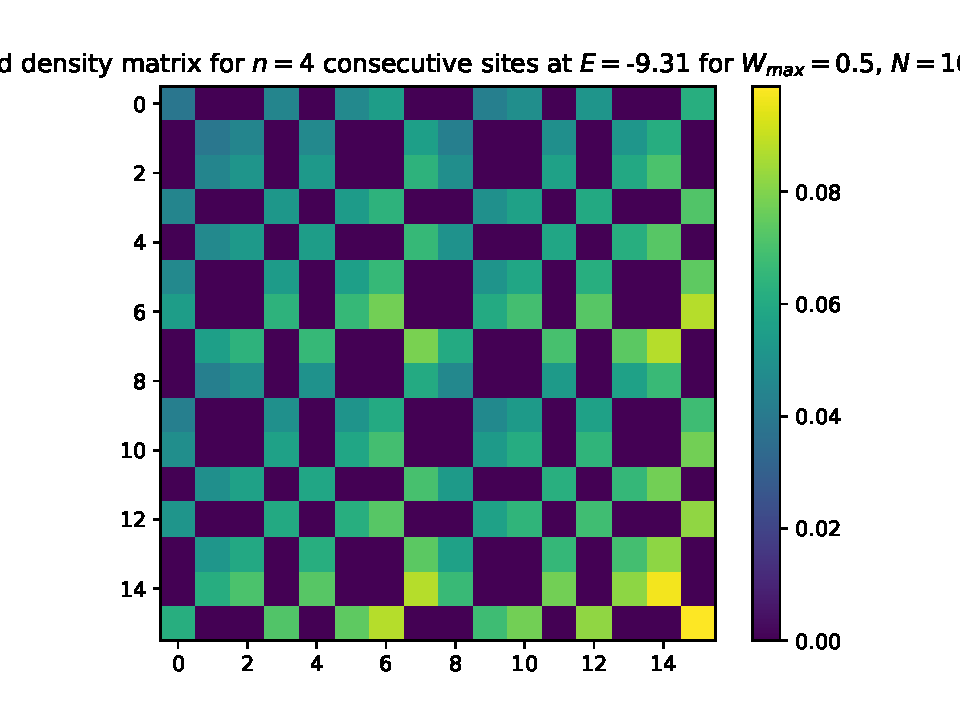
\includegraphics[width=\linewidth]{../results/groundstates/N10n4_trainingset_groundstate_Wmax0.5}
			\subcaption{Visualization of the ground state for an intermediate block size $n=4$ in the ergodic phase.}
		\end{subfigure}
		\begin{subfigure}[c]{0.45\textwidth}
			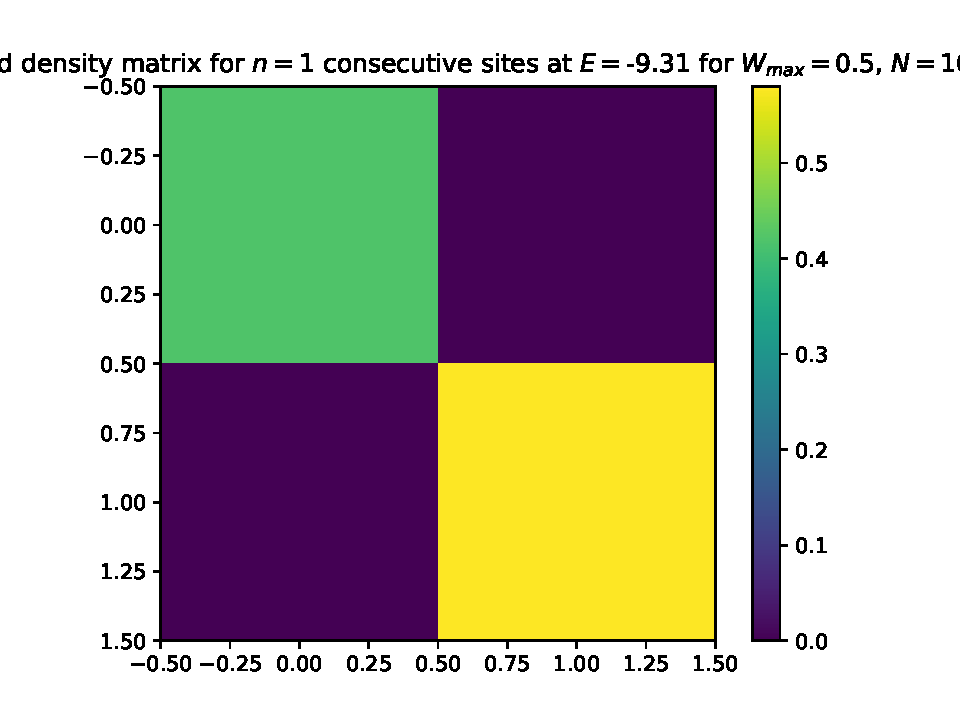
\includegraphics[width=\linewidth]{../results/groundstates/N10n1_trainingset_groundstate_Wmax0.5}
			\subcaption{Visualization of the ground state for the minimal block size $n=1$ in the ergodic phase.}
		\end{subfigure}
		\caption{Ground states for different block sizes $n$ and phases.}
		\label{fig:groundstates_erg}
	\end{figure}
\end{center}
%\twocolumngrid

The visual inspection indicates that the density matrix of the localized phase has a sharp maximum at the preferred state that is forced by the random disorder strength. The extended phase shows a sparse but certainly more even distribution, which reflects that some configurations are still more preferred than others induced by the coupling term in the Hamiltonian. The biggest maxima are likely still influenced by the random disorder strength. Another observation is that the density matrix reductions of the full ground state conserved these properties for $n>2$, when comparing $n=6$ to $n=\left[2,5\right]$. The similarity between the two phases gets smaller the smaller the block size $n$ gets. For $n=1$, one could argue that the density matrices are very similar, as they only deviate for half of the matrix elements. In conclusion, the ergodic reduced density matrix shows far more thermalization than the localized one.

\subsection{Model training}\label{sec:loss_acc}

Before we can predict the phase of a newly generated test set, we have to train the neural network with our available training data. For each system and block size a separate model was trained, as a different system size might influence the physical behavior due to open boundary conditions.

The neural networks are generated as a sequential keras model with the following configuration, as discussed in section \ref{sec:nn}: 
\begin{lstlisting}[language=Python]
model = models.Sequential()
if self.n > 3:
	filters = self.n*self.n
	model.add(layers.Conv2D(filters, (3, 3), activation='relu', input_shape=(np.shape(self.X_train[0])[0], np.shape(self.X_train[0])[1], 2)))
	model.add(layers.MaxPooling2D((4, 4)))
	model.add(layers.Dropout(rate=0.1))
	model.add(layers.Flatten())
else:
	model.add(layers.Flatten(input_shape=(np.shape(self.X_train)[1], np.shape(self.X_train)[1], 2)))
	model.add(layers.Dropout(rate=0.1))
	model.add(layers.Dense(32, activation='relu')),

model.add(layers.Dropout(rate=0.1))
model.add(layers.Dense(32, activation='relu'))
model.add(layers.Dense(1, activation='sigmoid'))
model.compile(optimizer='adam', loss='binary_crossentropy', metrics=['accuracy'])
\end{lstlisting}

To prevent over-fitting, $30$ \% of the training set was used for validation. To avoid a biased split, we relied on \texttt{sklearn}'s method \texttt{train\_test\_split} that samples randomly from the training set. Two dropout layers granted a better regularization, such that the training set was not overfitted.
	
The model training was executed by using a batch size of 70 and 100 epochs, where the batch size was limited by the CPU performance and no significant loss or accuracy improvements where noted after $>100$ epochs.

An example of the accuracy and loss dependency on the number of epochs for system size $L=8$, and block sizes $n=\{1, 6\}$ is presented below in Figure \ref{fig:accuracy_loss_epochs}.

\begin{figure}[h!]
	\centering
	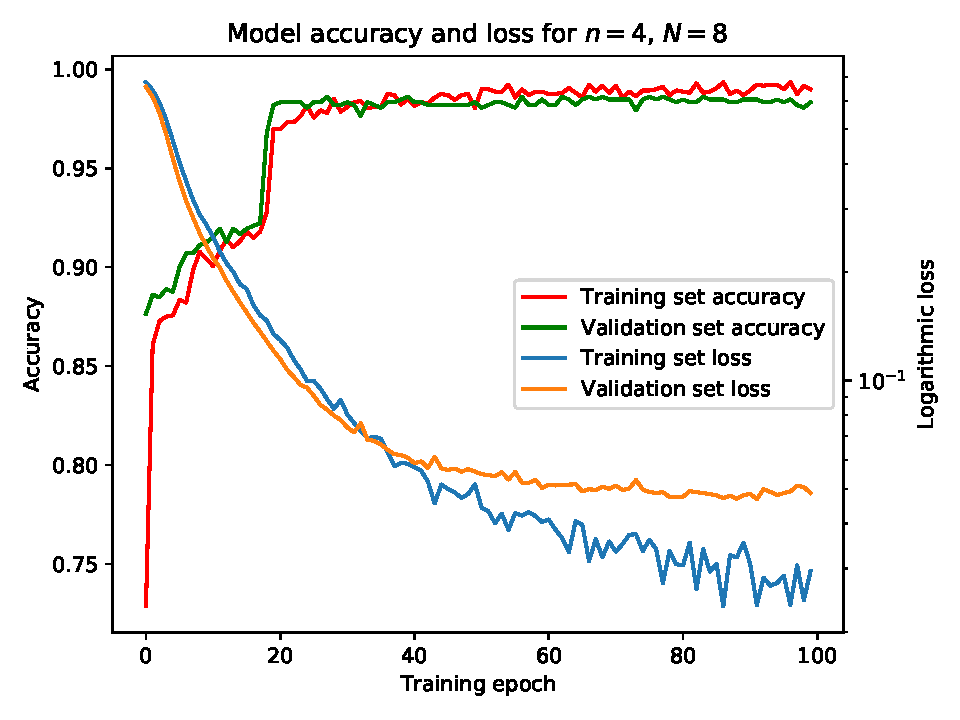
\includegraphics[width=\linewidth]{../results/accuracy_loss_epochs/N8n4_accuracy_loss_epochs}
	\caption{Accuracy and loss evolution over training epochs.}
	\label{fig:accuracy_loss_epochs}
\end{figure}

Figure \ref{fig:accuracy_loss_epochs} illustrates that the model is still not completely prone to overfitting. This can be accounted to the big model size in comparison to the sample size. Still, the loss stagnated at an acceptable optimum after 100 training epochs for all block and sytem sizes. The validation loss was the lowest for large system sizes and intermediate block sizes. 

\begin{figure}[h!]
	\centering
	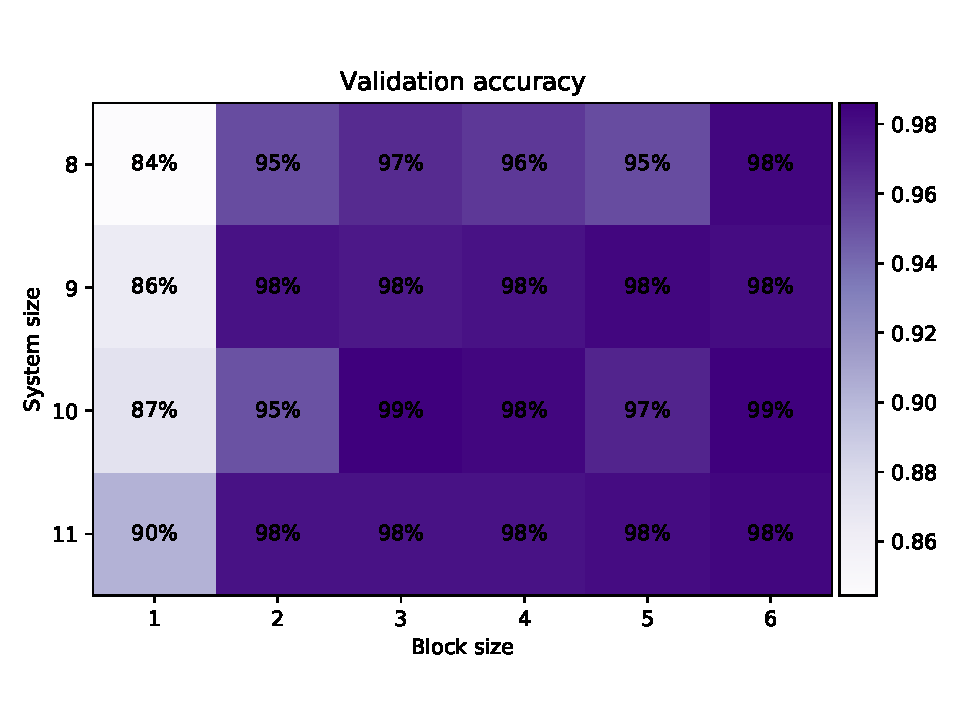
\includegraphics[width=\linewidth]{../results/accuracy_loss_epochs/all_validation_accuracy}
	\caption{Overview over the resulting accuracies on the validation set.}
	\label{fig:all_validation_accuracy}
\end{figure}

\begin{figure}
	\centering
	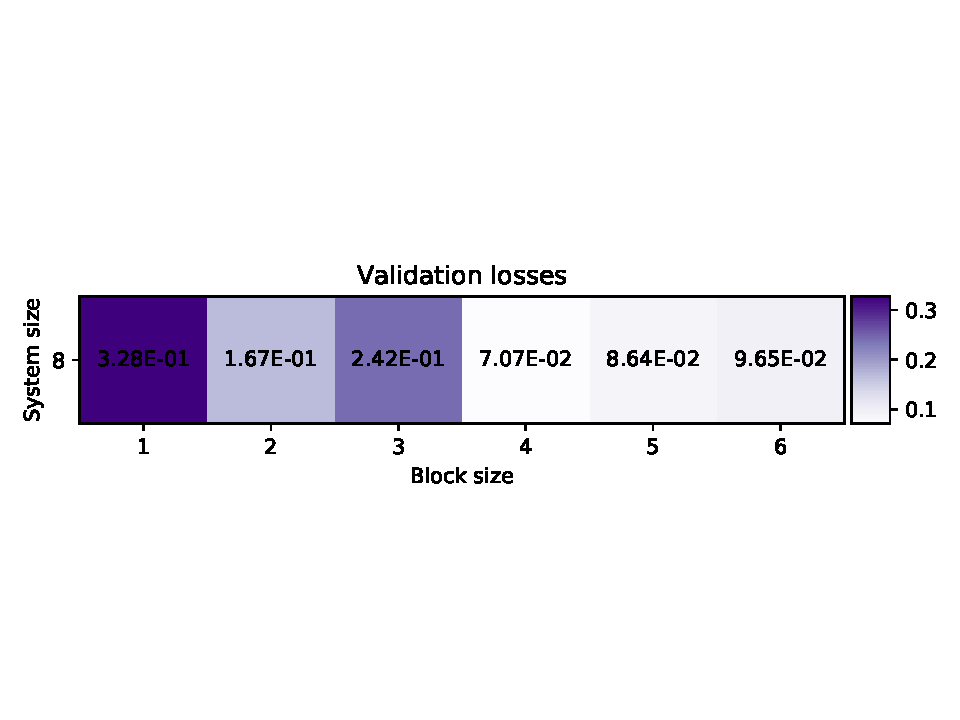
\includegraphics[width=\linewidth]{../results/accuracy_loss_epochs/all_validation_losses}
	\caption{Overview over the resulting losses on the validation set.}
	\label{fig:all_validation_accuracy}
\end{figure}

The validation losses in Figure \ref{fig:all_validation_accuracy} tell a similar story. Here, intermediate block sizes of $n=\{3, 4, 5, 6\}$ show the lowest validation loss. In the intermediate regime, the density matrices have a reasonable trade off between level of detail and number of weights in the neural network, since the first layer must match the input dimensions.

In conclusion, large system sizes and intermediate block sizes showed the best results. In addition, one can safely disregard predictions by models for block size $n=1$.

\subsection{Analysis of critical disorder strength}
\subsubsection{Dependency on block size}
At first, the testing set was generated. Following the parameter discussion in section \ref{sec:param}, we generated 180 samples for each $W\in\left[0,4\right]$, with step $\Delta W=0.5$, resulting in 1440 samples per system and block size. Afterwards, $W_c$ was obtained as described in section \ref{sec:wcextract}.
180 predicted phases are averaged at each point and plotted onto a heat map. $W_c$ is plotted in addition to that in Figure \ref{fig:wcextractn}.

%\onecolumngrid
\begin{center}
	\begin{figure}[hb!]
		\centering	
		\begin{subfigure}[c]{0.4\textwidth}
			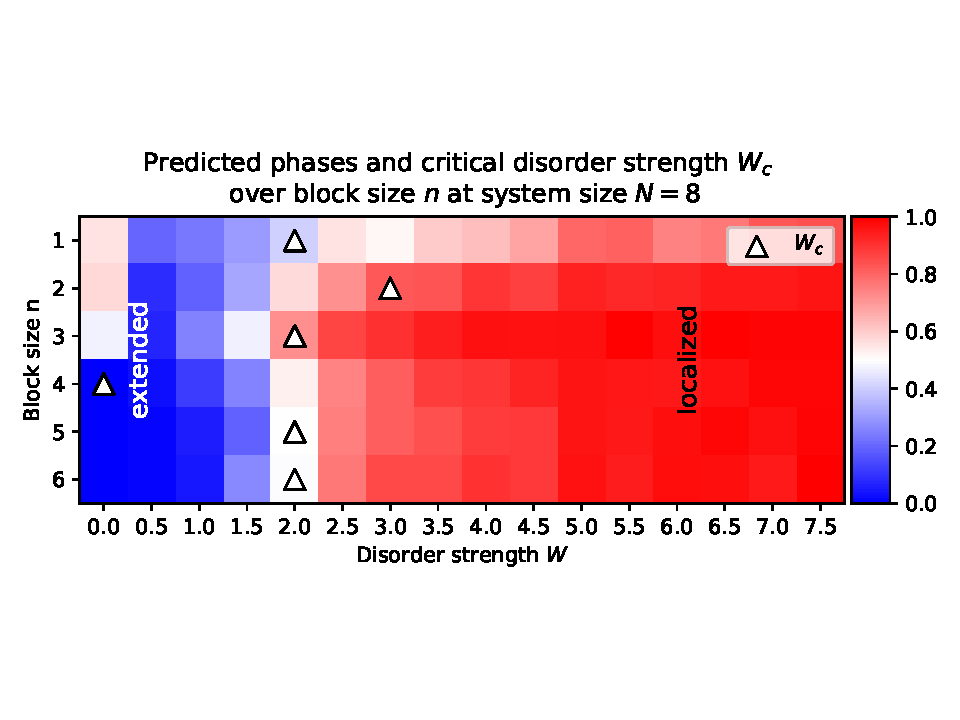
\includegraphics[width=\textwidth, trim={0 2cm 0 3cm},clip]{../results/Wc/N8_Wc_n_dependency.pdf}
			\subcaption{$L=8$}
		\end{subfigure}
		\begin{subfigure}[c]{0.4\textwidth}
			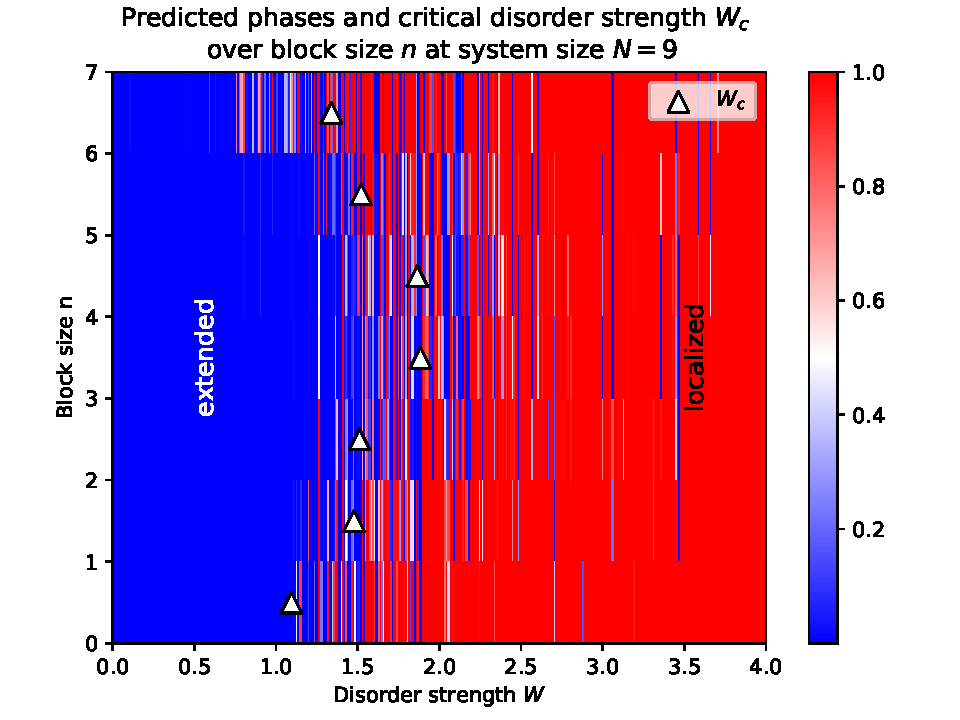
\includegraphics[width=\textwidth, trim={0 2cm 0 3cm},clip]{../results/Wc/N9_Wc_n_dependency.pdf}
			\subcaption{$L=9$}
		\end{subfigure}
	\end{figure}
	\begin{figure}[ht!]\ContinuedFloat
		\begin{subfigure}[c]{0.4\textwidth}
			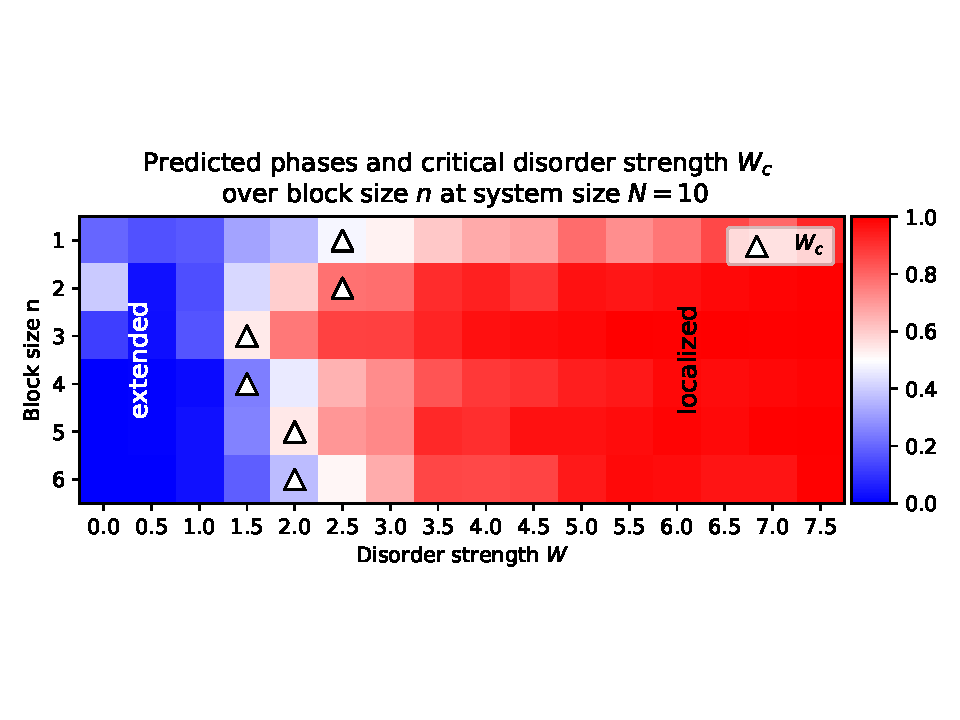
\includegraphics[width=\textwidth, trim={0 2cm 0 3cm},clip]{../results/Wc/N10_Wc_n_dependency.pdf}
			\subcaption{$L=10$}
		\end{subfigure}
		\begin{subfigure}[c]{0.4\textwidth}
			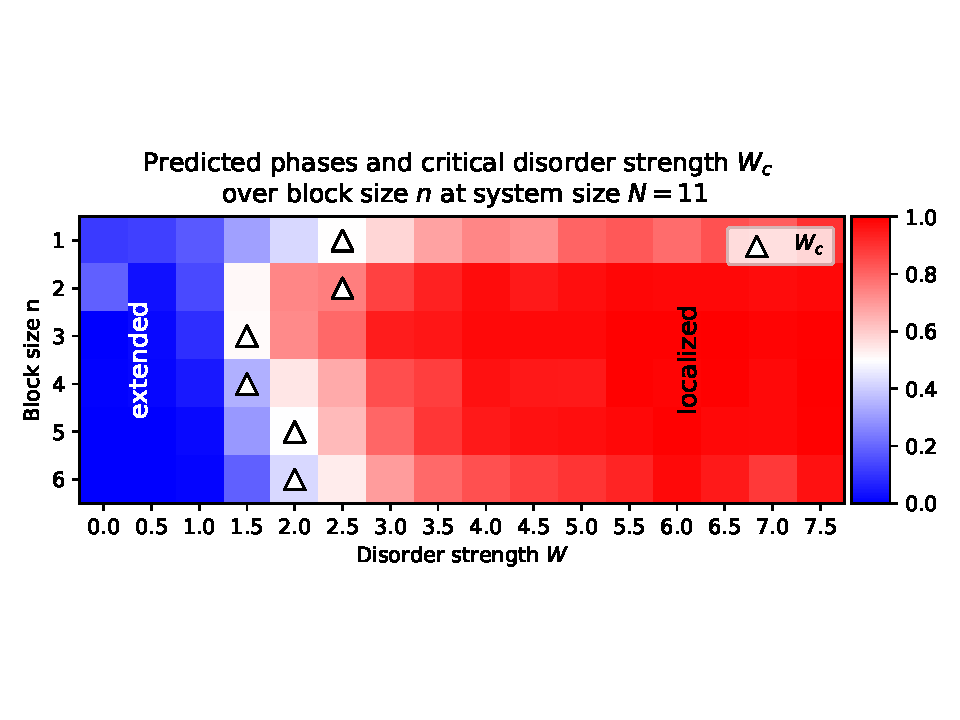
\includegraphics[width=\textwidth, trim={0 2cm 0 3cm},clip]{../results/Wc/N11_Wc_n_dependency.pdf}
			\subcaption{$L=11$}
		\end{subfigure}
		\begin{subfigure}[c]{0.4\textwidth}
			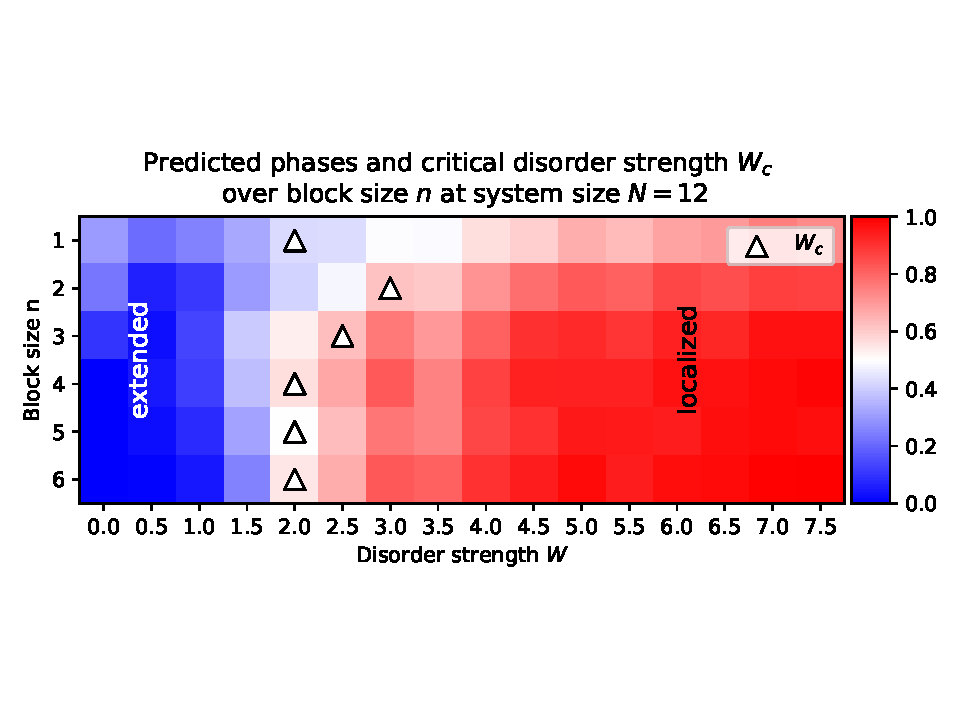
\includegraphics[width=\textwidth, trim={0 2cm 0 3cm},clip]{../results/Wc/N12_Wc_n_dependency.pdf}
			\subcaption{$L=12$}
		\end{subfigure}
		\caption{Dependency of the phase transition on block size $n$ for different system sizes.}
		\label{fig:wcextractn}
	\end{figure}
\end{center}
%\twocolumngrid

In conclusion, the predicted critical disorder strength $W_c$ decayed, when models with larger block sizes $n$ were used for prediction. On average, the extracted critical disorder strength was around $W_c=2.5J$.

\subsubsection{Dependency on system size}

Now, we rearrange the data, such that we can see the dependency on the system size by ordering each prediction set first by block size and plot them over system size. 

%\onecolumngrid
\begin{center}
	\begin{figure}[h]
		\centering	
		\begin{subfigure}[c]{0.4\textwidth}
			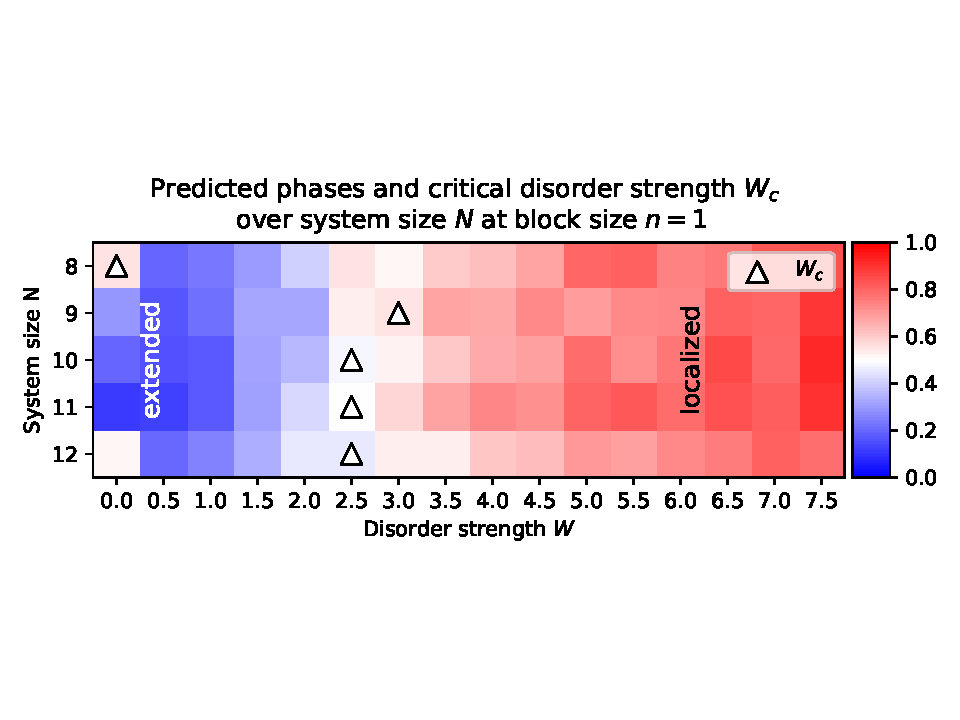
\includegraphics[width=\textwidth, trim={0 3cm 0 3cm},clip]{../results/Wc/n1_Wc_N_dependency.pdf}
			\subcaption{$n=1$}
		\end{subfigure}
		\begin{subfigure}[c]{0.4\textwidth}
			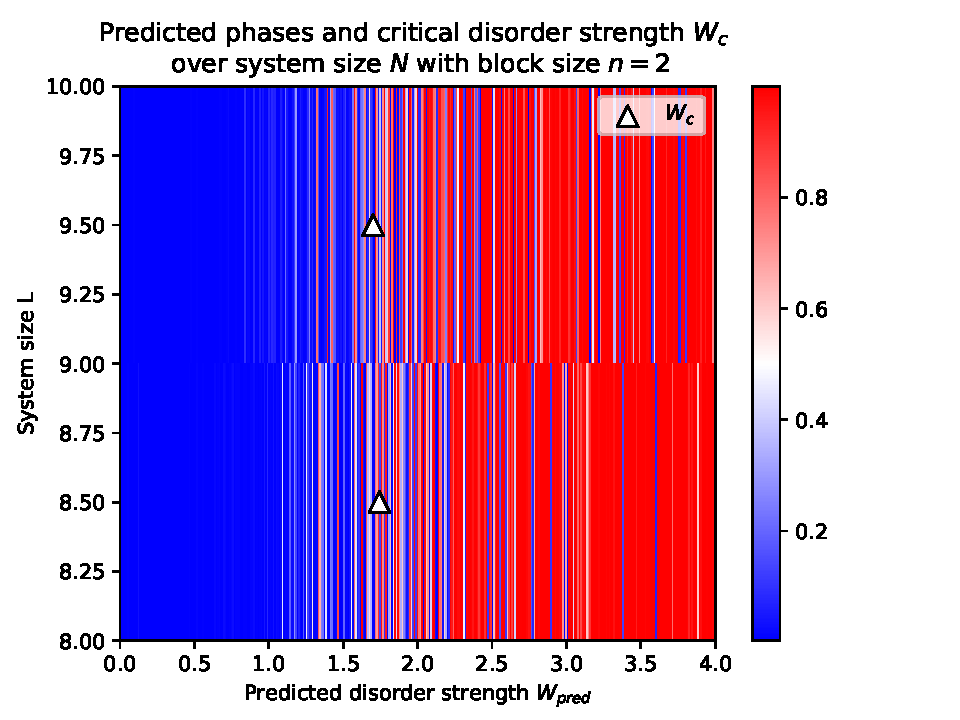
\includegraphics[width=\textwidth, trim={0 3cm 0 3cm},clip]{../results/Wc/n2_Wc_N_dependency.pdf}
			\subcaption{$n=2$}
		\end{subfigure}
		\begin{subfigure}[c]{0.4\textwidth}
			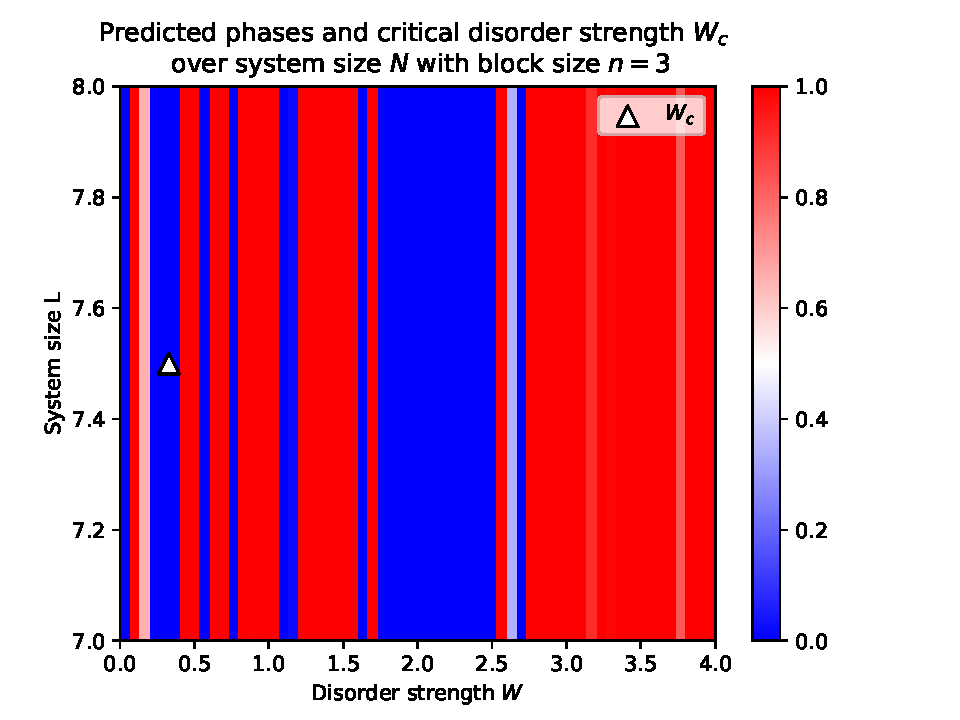
\includegraphics[width=\textwidth, trim={0 3cm 0 3cm},clip]{../results/Wc/n3_Wc_N_dependency.pdf}
			\subcaption{$n=3$}
		\end{subfigure}
		\begin{subfigure}[c]{0.4\textwidth}
			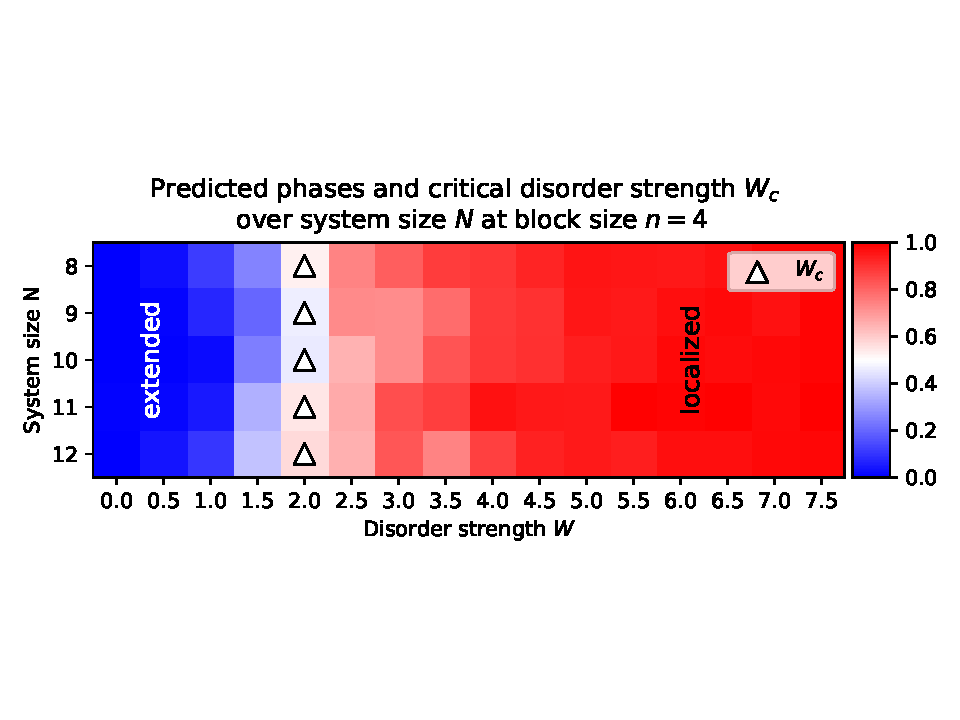
\includegraphics[width=\textwidth, trim={0 3cm 0 3cm},clip]{../results/Wc/n4_Wc_N_dependency.pdf}
			\subcaption{$n=4$}
		\end{subfigure}
		\begin{subfigure}[c]{0.4\textwidth}
			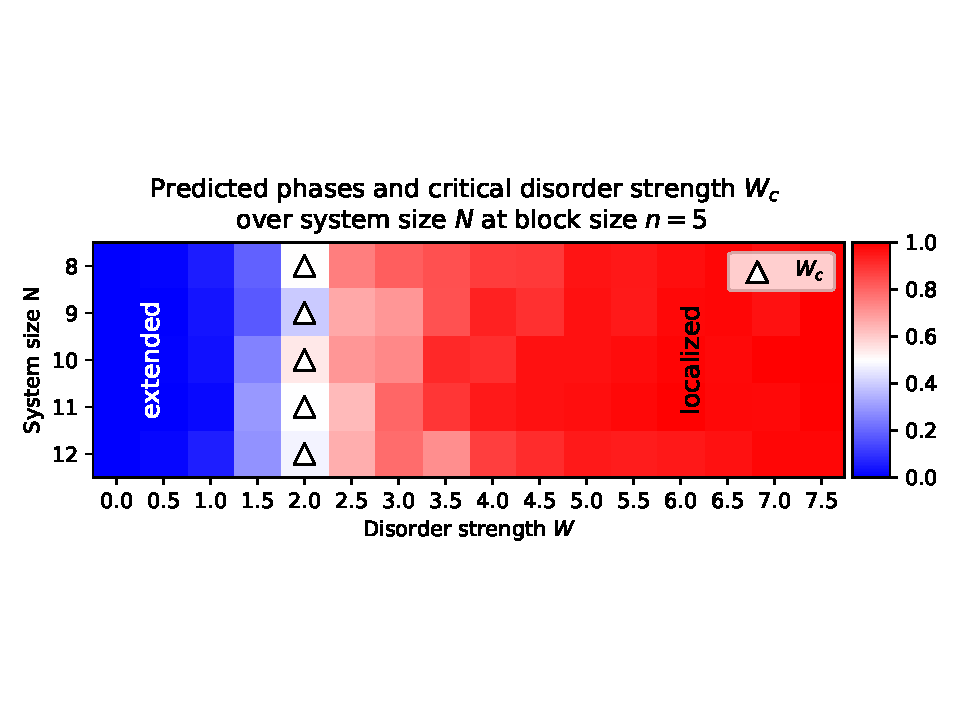
\includegraphics[width=\textwidth, trim={0 3cm 0 3cm},clip]{../results/Wc/n5_Wc_N_dependency.pdf}
			\subcaption{$n=5$}
		\end{subfigure}
	\end{figure}
	\begin{figure}[h]\ContinuedFloat
		\begin{subfigure}[c]{0.4\textwidth}
			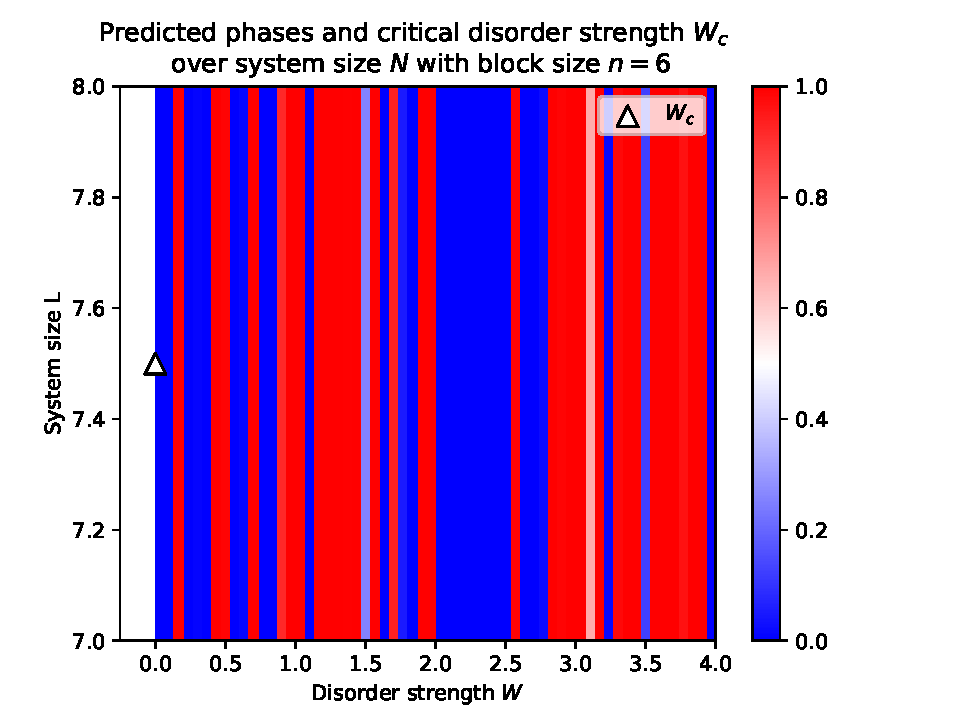
\includegraphics[width=\textwidth, trim={0 3cm 0 3cm},clip]{../results/Wc/n6_Wc_N_dependency.pdf}
			\subcaption{$n=6$}
		\end{subfigure}
		\caption{Dependency of the phase transition over system sizes $L$ for different block sizes $n$.}
		\label{fig:wcextract}
	\end{figure}
\end{center}
%\twocolumngrid

In comparison to the previous Figure, one can now see the dependency on the system size.
If we look at block size $n=1$, we can see again that the predicitons are not as well defined as for the other block sizes. This weakness can be tracked back to the low validation accuracy of $n=1$ models, which originated from the reduced density matrices being very similar for the ergodic and localized phase.

The plots are showing a near to constant dependency on the system size.
%W—>0 : reduced matrix : thermal density matrix , volume law entanglement
%W —> \infty : reduced density matrix: … , area law entanglement
%n is finite and large enough
%reduced density matrix would be different on two sides.

\section{Conclusion and Outlook}

In summary, the training set generation could be solved efficiently by employing the shift invert method in combination with the lanczos algorithm. The visual inspection of the density matrices showed that the ergodic phase is more thermalized than the localized phase as expected. Of course, the neural network still requires some tuning. Even though high accuracies were demonstrated, the validation loss was almost an order of magnitude higher than the training loss. An exception can be made for the block size $n=1$, which was found to be very hard to classify, as the thermalization did not have big enough of an impact to the input data.
However, the predicitons for intermediate disorder strength showed that a region for the phase transition could successfully be found for all block and system sizes. The classification accuracy outside of the phase transition was almost 100\%. 

Finally, the extracted critical disorder was hard to classify for a block size of $n=1$, and did not vary much for block sizes $n=\{4,5,6\}$. In the system size analysis, block size $n=4$ had the least deviations. In the analysis no clear trend was found with respect to finite size scaling. This would probably change if more effort on training set generation could be made. The here presented results can completely be generated within 24h on an average computer, which sets a clear constraint.

Still, a phase change could be consistently observed around $W_c=2.5$, deviating slightly from the result $W_c\approx3.6$ in Luitz et al. 2015 for larger system up to $L=22$.\cite{Luitz2015} It is expected that smaller systems with open boundary conditions show a smaller disorder strength, as fluctuations are not suppressed as much.

\bibliography{zotero}
%\bibliography{bibsamp}% Produces the bibliography via BibTeX.

\newpage
\appendix


\begin{widetext}
\section{Code listing} \label{app:codes}
The process can be broken down into five different steps, which can be all be executed through a main function, but can also be run separately: Generation of the training set, model training, generation if the testing set, generating predictions. Every file serves a number of different purposes as listed below. In general, the time for each step is estimated and logged to the console, such that the user can easily narrow down the parameter range for his own system.

To replicate the results, you can access the whole code and all plots at \url{https://gitlab.lrz.de/phkrueger/final-project-ph2264.git}. The tutors of PH2264 have been given guest access. Interested readers will be given access by contacting me via \url{ph.krueger@tum.de}.

\begin{enumerate}
	\item \textbf{main.py}: Executes the whole pipeline.
	\item \textbf{generate\_training\_set.py}: Here, the training set is generated and some example plots of ground states are saved to the results folder. The training sets are saved in the \texttt{training\_sets} folder, where they are numbered with their system and block size.
	\item \textbf{ed.py}: The training set is generated by using the functions from the tutorial. A new function was added that generates the Hamiltonian using the random local disorder strength.
	\item \textbf{dataset\_preparation.py}: While this file contains many important functions to preprocess and label the training and testing sets and load and save functions, it also has a method that plots the visualizations of a few ground states.
	\item \textbf{model\_save\_train.py}: First, models are generated that automatically match the input data of different block sizes $n$, afterwards, they are trained with a certain amount of epochs and batch sizes. The history of the validation and accuracy is plotted individually into the results folder.
	\item \textbf{generate\_test\_set.py}: A set of reduced density matrices for ground states in the intermediate regime is generated.
	\item \textbf{generate\_predictions.py}: The test sets are fed into the trained machine learning models. The predicted phases are averaged for every W, n, N combination and saved into a prediction dataset.
	\item \textbf{plot\_wc\_dependency.py}: The predictions are loaded, we extract $W_c$ and plot everything together as a heat map over system and block sizes.
\end{enumerate}

\subsection{Pipeline execution}
\lstinputlisting[language=Python]{../main.py}

\subsection{Training set generation}
\lstinputlisting[language=Python]{../generate_training_set.py}

\subsection{Exact diagonalization}
\lstinputlisting[language=Python]{../ed.py}

\subsection{Dataset Preparation}
\lstinputlisting[language=Python]{../dataset_preparation.py}

\subsection{Model Training}
\lstinputlisting[language=Python]{../model_save_train.py}

\subsection{Test set generation}
\lstinputlisting[language=Python]{../generate_test_set.py}

\subsection{Prediction}
\lstinputlisting[language=Python]{../generate_predictions.py}

\subsection{Evaluation of $W_c$}
\lstinputlisting[language=Python]{../plot_wc_dependency.py}



%\begin{lstlisting}[language=Python]
%%\include{file}
%\include{}
%\end{lstlisting}
\end{widetext}



\end{document}
